\appendix
\appendixpage
\renewcommand{\thesection}{A.\arabic{section}}
\addappheadtotoc

\section{Recovery Figures}
\label{appendix:bitmap-errors}

To visually demonstrate some limitations of this error correction scheme, the following figures show the use of Reed-Solomon codes to repair bitmap images.

Figure (a) has 12966 errors and can be repaired, yet figure (b) has only 3288 errors and cannot be repaired.
This is because the errors in figure (a) are one contiguous burst, whereas the errors in figure (b) are many small bursts spread across the image, damaging more blocks than in figure (a).

\begin{figure}[H]
    \centering
    \begin{subcaptionbox}{A recoverable bitmap image with one corrupt area.}
        {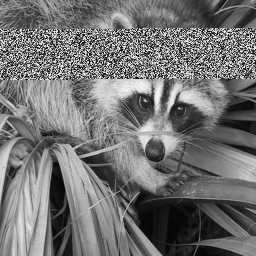
\includegraphics[width=0.3\textwidth]{face_2.png}}
    \end{subcaptionbox}
    \hfill
    \begin{subcaptionbox}{An unrecoverable bitmap image with many small corrupt areas.}
        {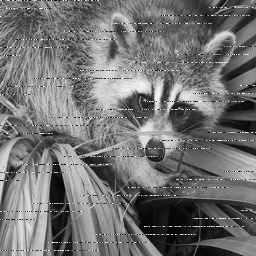
\includegraphics[width=0.3\textwidth]{face_3.png}}
    \end{subcaptionbox}
    \hfill
    \begin{subcaptionbox}{Figure (a), repaired.}
        {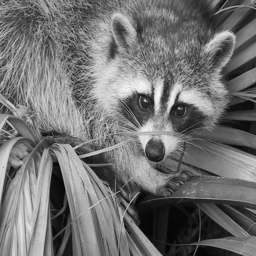
\includegraphics[width=0.3\textwidth]{face_2_repaired.png}}
    \end{subcaptionbox}
    
    \caption{Image source: \texttt{scipy.datasets.face} (derived from \url{https://pixnio.com/fauna-animals/raccoons/raccoon-procyon-lotor})}
\end{figure}

\clearpage

\subsection{Image Generation Script}

\begin{tiny}
\lstinputlisting[language=Python, showstringspaces=false]{generate_figures.py}
\end{tiny}

\clearpage

\section{Dependencies}

\label{appendix:dependencies}

The following Rust libraries were used in the implementation:

\begin{itemize}
    \item \texttt{fastrand} - Random number generation for testing.
    \item \texttt{blake3} - Hashing for error detection.
    \item \texttt{crossbean-channel} - Channels for communication between threads. Although the standard library provides channels, multi-producer multi-consumer channels are not stabilized yet (as of Rust 1.87.0).
    \item \texttt{indicatif} - Terminal progress bars.
    \item \texttt{memmap2} - Cross-platform memory mapped I/O.
    \item \texttt{num\_cpus} - Obtains of CPU cores for automatically selecting number of threads.
    \item \texttt{positioned-io} - Cross-platform random access file I/O.
    \item \texttt{sysinfo} - Obtains available memory for automatically selecting number of codes to process at once.
\end{itemize}
